\documentclass[a4paper,12pt]{article}
\usepackage[utf8]{inputenc}
\usepackage[spanish]{babel}
\usepackage{color}
\usepackage{parskip}
\usepackage{graphicx}
\usepackage{multirow}
\usepackage{listings}
\usepackage{vmargin}
\usepackage{float}
\graphicspath{ {imagenes/} }
\definecolor{mygreen}{rgb}{0,0.6,0}
\definecolor{lbcolor}{rgb}{0.9,0.9,0.9}
\usepackage{epstopdf}

\setpapersize{A4}
\setmargins{2.5cm}       % margen izquierdo
{1.5cm}                        % margen superior
{16.5cm}                      % anchura del texto
{23.42cm}                    % altura del texto
{10pt}                           % altura de los encabezados
{1cm}                           % espacio entre el texto y los encabezados
{0pt}                             % altura del pie de página
{2cm}     

\lstset{
backgroundcolor=\color{lbcolor},
    tabsize=4,    
%   rulecolor=,
    language=[GNU]C++,
        basicstyle=\tiny,
        aboveskip={1.5\baselineskip},
        columns=fixed,
        showstringspaces=false,
        extendedchars=false,
        breaklines=true,
        prebreak = \raisebox{0ex}[0ex][0ex]{\ensuremath{\hookleftarrow}},
        frame=single,
        showtabs=false,
        showspaces=false,
        showstringspaces=false,
        identifierstyle=\ttfamily,
        keywordstyle=\color[rgb]{0,0,1},
        commentstyle=\color[rgb]{0.026,0.112,0.095},
        stringstyle=\color{red},
        numberstyle=\color[rgb]{0.205, 0.142, 0.73},
%        \lstdefinestyle{C++}{language=C++,style=numbers}’.
}

\begin{document}

Programar los cinco métodos iterativos planteados en clase, para dar solución a las siguientes ecuaciones:

\begin{itemize}
 \item $x-x^{x-cosx} = 0$
 \item $x-cos(senx) = 0$
 \item $x^5 - 3x^3 - 2x^2 + 2 = x$
\end{itemize}

\textbf{NOTA: }Dar la respuesta más próxima a cero.

\section{Código}

  \subsection{formulas.h}
   
  Contiene funciones necesarias en todos los métodos.
  
  \begin{lstlisting}
#ifndef FORMULAS_H
#define FORMULAS_H

#include <iostream>
#include <cmath>

using namespace std;

typedef long double Number;

Number ErrorRelativo(Number x, Number xs){
	return abs(xs - x) / abs(x);
}

Number ErrorAbsoluto(Number x, Number xs){
	return abs(xs - x);
}

#endif
  \end{lstlisting}
  
  \subsection{MetodosCerrados.cpp}
  
  Contiene la función \textbf{Metodo Cerrado()} que sirve tanto para el Método de Bisección como para el Método
  de Falsa posición, teniendo el mismo algoritmo con una única diferencia: la forma de calcular su siguiente aproximación.
  Para el Método de Bisección se utiliza la función \textbf{Bisección()}, mientras que para el método de Falsa podición se 
  utiliza la función \textbf{FalsaPosicion()}. La ecuación que se quiere resolver debe ser programada dentro de la función
  \textbf{Funcion()}. \\
  El resultado del programa es un archivo .csv con una tabla con los resultados, que podrá 
  ser abierto con cualquier editor de tablas de datos(Excel ó LibreOffice).
  
  \begin{lstlisting}
#include <iostream>
#include <fstream>
#include <cmath>
#include "formulas.h"

/// rjhancco@impa.br

using namespace std;

enum Tipos{BISECCION,FALSA_POSICION};

Number Biseccion(Number a, Number b){
	return (a + b) / 2;
}

Number FalsaPosicion(Number a, Number b, Number fa, Number fb){
	return a - ((b-a)/(fb-fa)) * fa;
}

Number Funcion(Number x){
	return x - pow(x,x-cos(x));
}

bool MetodoCerrado(Number a, Number b, string file, Number(*f)(Number), int tipo, Number presicion, int n){
	if(f(a) * f(b) >= 0 or tipo < BISECCION or tipo > FALSA_POSICION) return false;
	string fi = file + ".csv";
	ofstream archivo(fi);
	if(archivo.fail()) return false;
	archivo.precision(15);
	archivo<<"\"i\",\"ai\",\"bi\",\"ri\",\"f(ri)\",\"f(ai)\",\"f(b1)\""<<endl;
	Number r = 0;
	Number fr = 0;
	Number fa = 0;
	Number fb = 0;
	Number r_anterior= 0;
	int i = 0;
	do{
		r_anterior = r;
		fa = f(a);
		fb = f(b);
		if(tipo == BISECCION) r = Biseccion(a,b);
		else r = FalsaPosicion(a,b,fa,fb);
		fr = f(r);
		archivo<<i<<","<<a<<","<<b<<","<<r<<","<<fr<<","<<fa<<","<<fb<<endl;
		if(fa * fr < 0) b = r;
		else a = r;
		i++;
	}while((ErrorAbsoluto(r_anterior, r) > presicion and i != n) or i == 1);
	archivo<<"\"Resultado Final\","<<r<<endl;
	archivo.close();
	return true;
}

int main(){
	Number (*f)(Number) = Funcion;
	Number a;
	Number b;
	Number presicion;
	int n;
	int tt;
	string file;
	cout<<"Ingrese a->";
	cin>>a;
	cout<<"Ingrese b->";
	cin>>b;
	cout<<"BISECCION (1) o FALSA POSICION (2)";
	cin>>tt;
	cout<<"Ingrese la precision->";
	cin>>presicion;
	cout<<"Ingrese la n->";
	cin>>n;
	cout<<"Nombre del archivo donde quiere que salga la tabla->";
	cin>>file;
	if(!MetodoCerrado(a,b,file,f,tt-1,presicion,n)) cout<<"Hubo un Problema"<<endl;
	else cout<<"Archivo generado correctamente"<<endl;
}
  \end{lstlisting}
  
  \subsection{MetodosAbiertos.cpp}
  
  En este caso hay una función para cada método restante: Método de la Secante(\textbf{MetodoSecante()})), 
  Método de Newton(\textbf{MetododeNewton\_A()}), Método de Newton con derivada aproximada(\textbf{MetodoNewton\_B()}).
  La ecuación que se quiere resolver debe ser programada dentro de la función
  \textbf{funcion()}.\\
  El resultado del programa es un archivo .csv con una tabla con los resultados, que podrá 
  ser abierto con cualquier editor de tablas de datos(Excel ó LibreOffice).
  
  \begin{lstlisting}
#include <iostream>
#include <fstream>
#include <cmath>
#include "formulas.h"

using namespace std;

// x-x^(x-cosx)  = 0
// x - cos(sen(x)) = 0
// x^5 - 3x^3 - 2x^2 + 2 = x

enum Tipos{SECANTE = 1, NEWTON_A, NEWTON_B};

Number funcion(Number x){
	return x*x*x - 2;
}

Number _funcion(Number x){
	return 3 * x*x;
}

Number _MetodoSecante(Number r0, Number r1, Number fr0, Number fr1){
	return r0-((r1-r0)/(fr1-fr0))*fr0;
}

Number _MetodoNewton_A(Number r, Number fr, Number f_r){
	return r - (fr/f_r);
}

Number _MetodoNewton_B(Number r, Number fr, Number frh, Number h){
	return r * ((fr * h)/(frh - fr));
}

void MetodoSecante(Number r0, Number r1, Number(*f)(Number), int n, Number presicion, string fi){
	string file = fi + ".csv";
	ofstream archivo(file);
	Number fr0 = f(r0);
	Number fr1 = f(r1);
	Number fr2 = 0;
	Number r2 = 0;
	int i = 1;
	archivo<<"\"i\",\"ri-1\",\"ri\",\"f(ri-1)\",\"f(ri)\",\"ri+1\",\"f(r1+1)\""<<endl;
	do{
		r2 = _MetodoSecante(r0,r1,fr0,fr1);
		fr2 = f(r2);
		archivo<<i<<","<<r0<<","<<r1<<","<<fr0<<","<<fr1<<","<<r2<<","<<fr2<<endl;
		r0 = r1;
		r1 = r2;
		fr0 = fr1;
		fr1 = fr2;
		i++;
	}while((ErrorAbsoluto(r0,r1) > presicion and i != n) or i == 2);
	archivo<<"\"Resultado Final\","<<r1<<endl;
	archivo.close();
}


void MetodoNewton_A(Number r, Number(*f)(Number), Number(*df)(Number), Number presicion, int n, string fi){
	string file = fi + ".csv";
	ofstream archivo(file);
	Number fr = 0;
	Number f_r = 0;
	Number r2 = 0;
	Number r_anteriror;
	int i = 0;
	archivo<<"\"i\",\"ri\",\"f(ri)\",\"f'(r1)\",\"ri+1\""<<endl;
	do{
		r_anteriror = r;
		fr = f(r);
		f_r = df(r);
		r2 = _MetodoNewton_A(r,fr,f_r);
		archivo<<i<<","<<r<<","<<fr<<","<<f_r<<","<<r2<<endl;
		r = r2;
		i++;
	}while((ErrorAbsoluto(r_anteriror, r) > presicion and i != n)or i == 1);
	archivo<<"\"Resultado actual\","<<r<<endl;
	archivo.close();
}

void MetodoNewton_B(Number r, Number(*f)(Number), Number h, Number presicion, int n, string fi){
	string file = fi + ".csv";
	ofstream archivo(file);
	Number fr = 0;
	Number frh = 0;
	Number r2 = 0;
	Number r_anteriror = 0;
	int i = 0;
	archivo<<"\"i\",\"ri\",\"f(ri)\",\"f(ri+h)\",\"ri+1\""<<endl;
	do{
		r_anteriror = r;
		fr = f(r);
		frh = f(r+h);
		r2 = _MetodoNewton_B(r,fr,frh,h);
		archivo<<i<<","<<r<<","<<fr<<","<<frh<<","<<r2<<endl;
		r = r2;
		i++;
	}while((ErrorAbsoluto(r_anteriror, r) > presicion and i != n)or i == 1);
	archivo<<"\"Resultado actual\","<<r<<endl;
	archivo.close();
}

int main(){
	Number r0;
	int n;
	Number presicion;
	Number (*f)(Number) = funcion;
	string file;
	int tipo;
	cout<<"Que metodo quiere usar->Secante(1) - Newton_A (2) - Newton_B (3)";
	cin>>tipo;
	cout<<"Ingrese el r0->";
	cin>>r0;
	cout<<"Ingrese el la presicion->";
	cin>>presicion;
	cout<<"Ingrese n->";
	cin>>n;
	cout<<"Ingrese nombre del archivo dende saldra la tabla->";
	cin>>file;
	if(tipo == SECANTE){
		Number r1;
		cout<<"Ingrese el r1->";
		cin>>r1;
		MetodoSecante(r0,r1,f,n,presicion,file);
		cout<<"Archivo generado correctamente"<<endl;
	}
	else if(tipo == NEWTON_A){
		Number (*df)(Number) = _funcion;
		MetodoNewton_A(r0,f,df,presicion,n,file);
		cout<<"Archivo generado correctamente"<<endl;
	}
	else if(tipo == NEWTON_B){
		Number h;
		cout<<"Ingrese el h->";
		cin>>h;
		MetodoNewton_B(r0,f,h,presicion,n,file);
		cout<<"Archivo generado correctamente"<<endl;
	}
	else cout<<"Ocurrio algo"<<endl;
}
  \end{lstlisting}

  \subsection{PuntoFijo.cpp}
  
  \begin{lstlisting}
#include <iostream>
#include <fstream>
#include <cmath>
#include "formulas.h"

using namespace std;

Number funcion(Number x){
	return x - pow(x,x-cos(x));
	//return x - cos(sin(x));
	//return pow(x,5) - 3 * pow(x,3) - 2 * x * x + 2 - x;
	//return 1 - (x*x/4);
}

Number _funcion(Number x){
	return pow(x,x-cos(x));
	//return x - cos(sin(x)) + x;
	//return pow(x,5) - 3 * pow(x,3) - 2 * x * x + 2 - x + x;
	//return 1 + x -(x*x/4);
}

void MetodoPuntoFijo(Number(*f)(Number),Number(*g)(Number), Number r, string fi, Number n, Number presicion){
	string file = fi + ".csv";
	ofstream archivo(file);
	Number fr = 0;
	Number gr = 0;
	Number i = 0;
	Number r_anterior = 0;
	archivo<<"\"i\",\"ri\",\"f(ri)\",\"g(ri)\""<<endl;
	do{
		r_anterior = r;
		fr = f(r);
		gr = g(r);
		archivo<<i<<","<<r<<","<<fr<<","<<gr<<endl;
		r = gr;
		i++;
	}while((ErrorAbsoluto(r_anterior,r) > presicion and i != n) or i == 1);
	archivo<<"\"Resultado Final\","<<r<<endl;
	archivo.close();
	cout<<"Archivo generado correctamente"<<endl;
}

int main(){
	Number(*f)(Number) = funcion;
	Number(*g)(Number) = _funcion;
	Number r;
	Number n;
	Number presicion;
	string file;
	cout<<"Ingrese su r0->";
	cin>>r;
	cout<<"Ingrese su n->";
	cin>>n;
	cout<<"Ingrese la presicion->";
	cin>>presicion;
	cout<<"Ingrese el nombre del archivo->";
	cin>>file;
	MetodoPuntoFijo(f,g,r,file,n,presicion);
}
  \end{lstlisting}

  
  
  
  \section{Soluciones}
  
    Todas las pruebas con todos los métodos se hicieron con una $presicion$ igual a $10^{-6}$ y un $n$ igual a $100$. 
  
    \subsection{Gráficas}
    
    \begin{itemize}
     \item $x-x^{x-cosx} = 0$
     
     \begin{figure}[h]
      \centering
      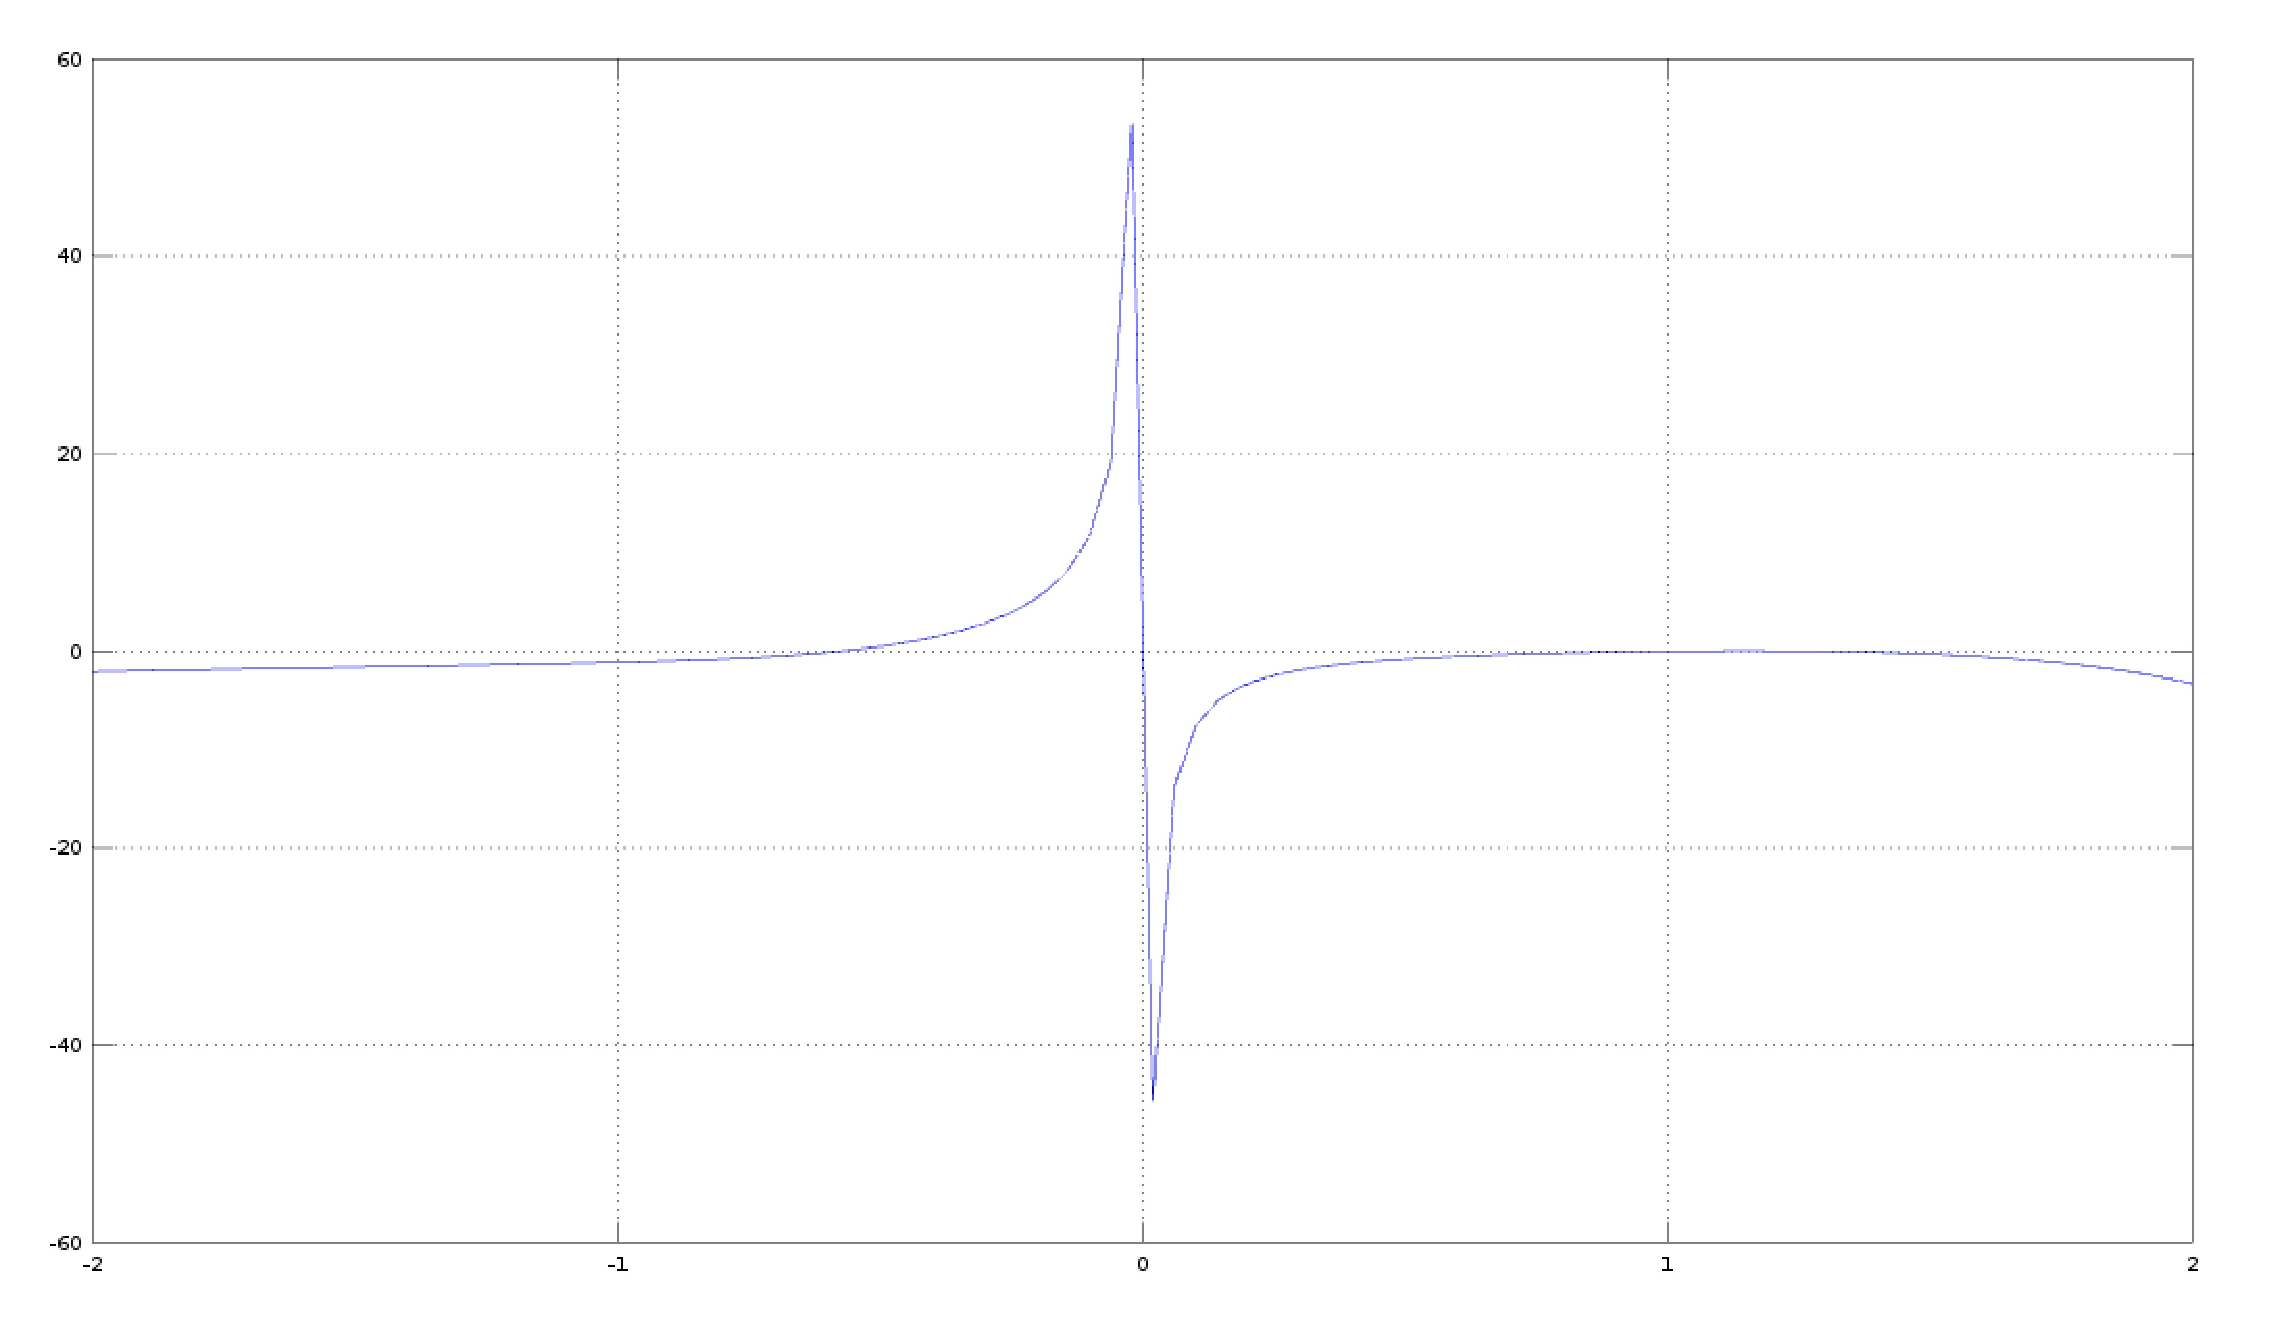
\includegraphics[scale = 0.3]{1.eps}
     \end{figure}

     
     \item $x-cos(senx) = 0$
     
     \begin{figure}[h]
      \centering
      \includegraphics[scale = 0.3]{2.eps}
     \end{figure}
     
     \newpage
     
     \item $x^5 - 3x^3 - 2x^2 + 2 = x$
     
     \begin{figure}[h]
      \centering
      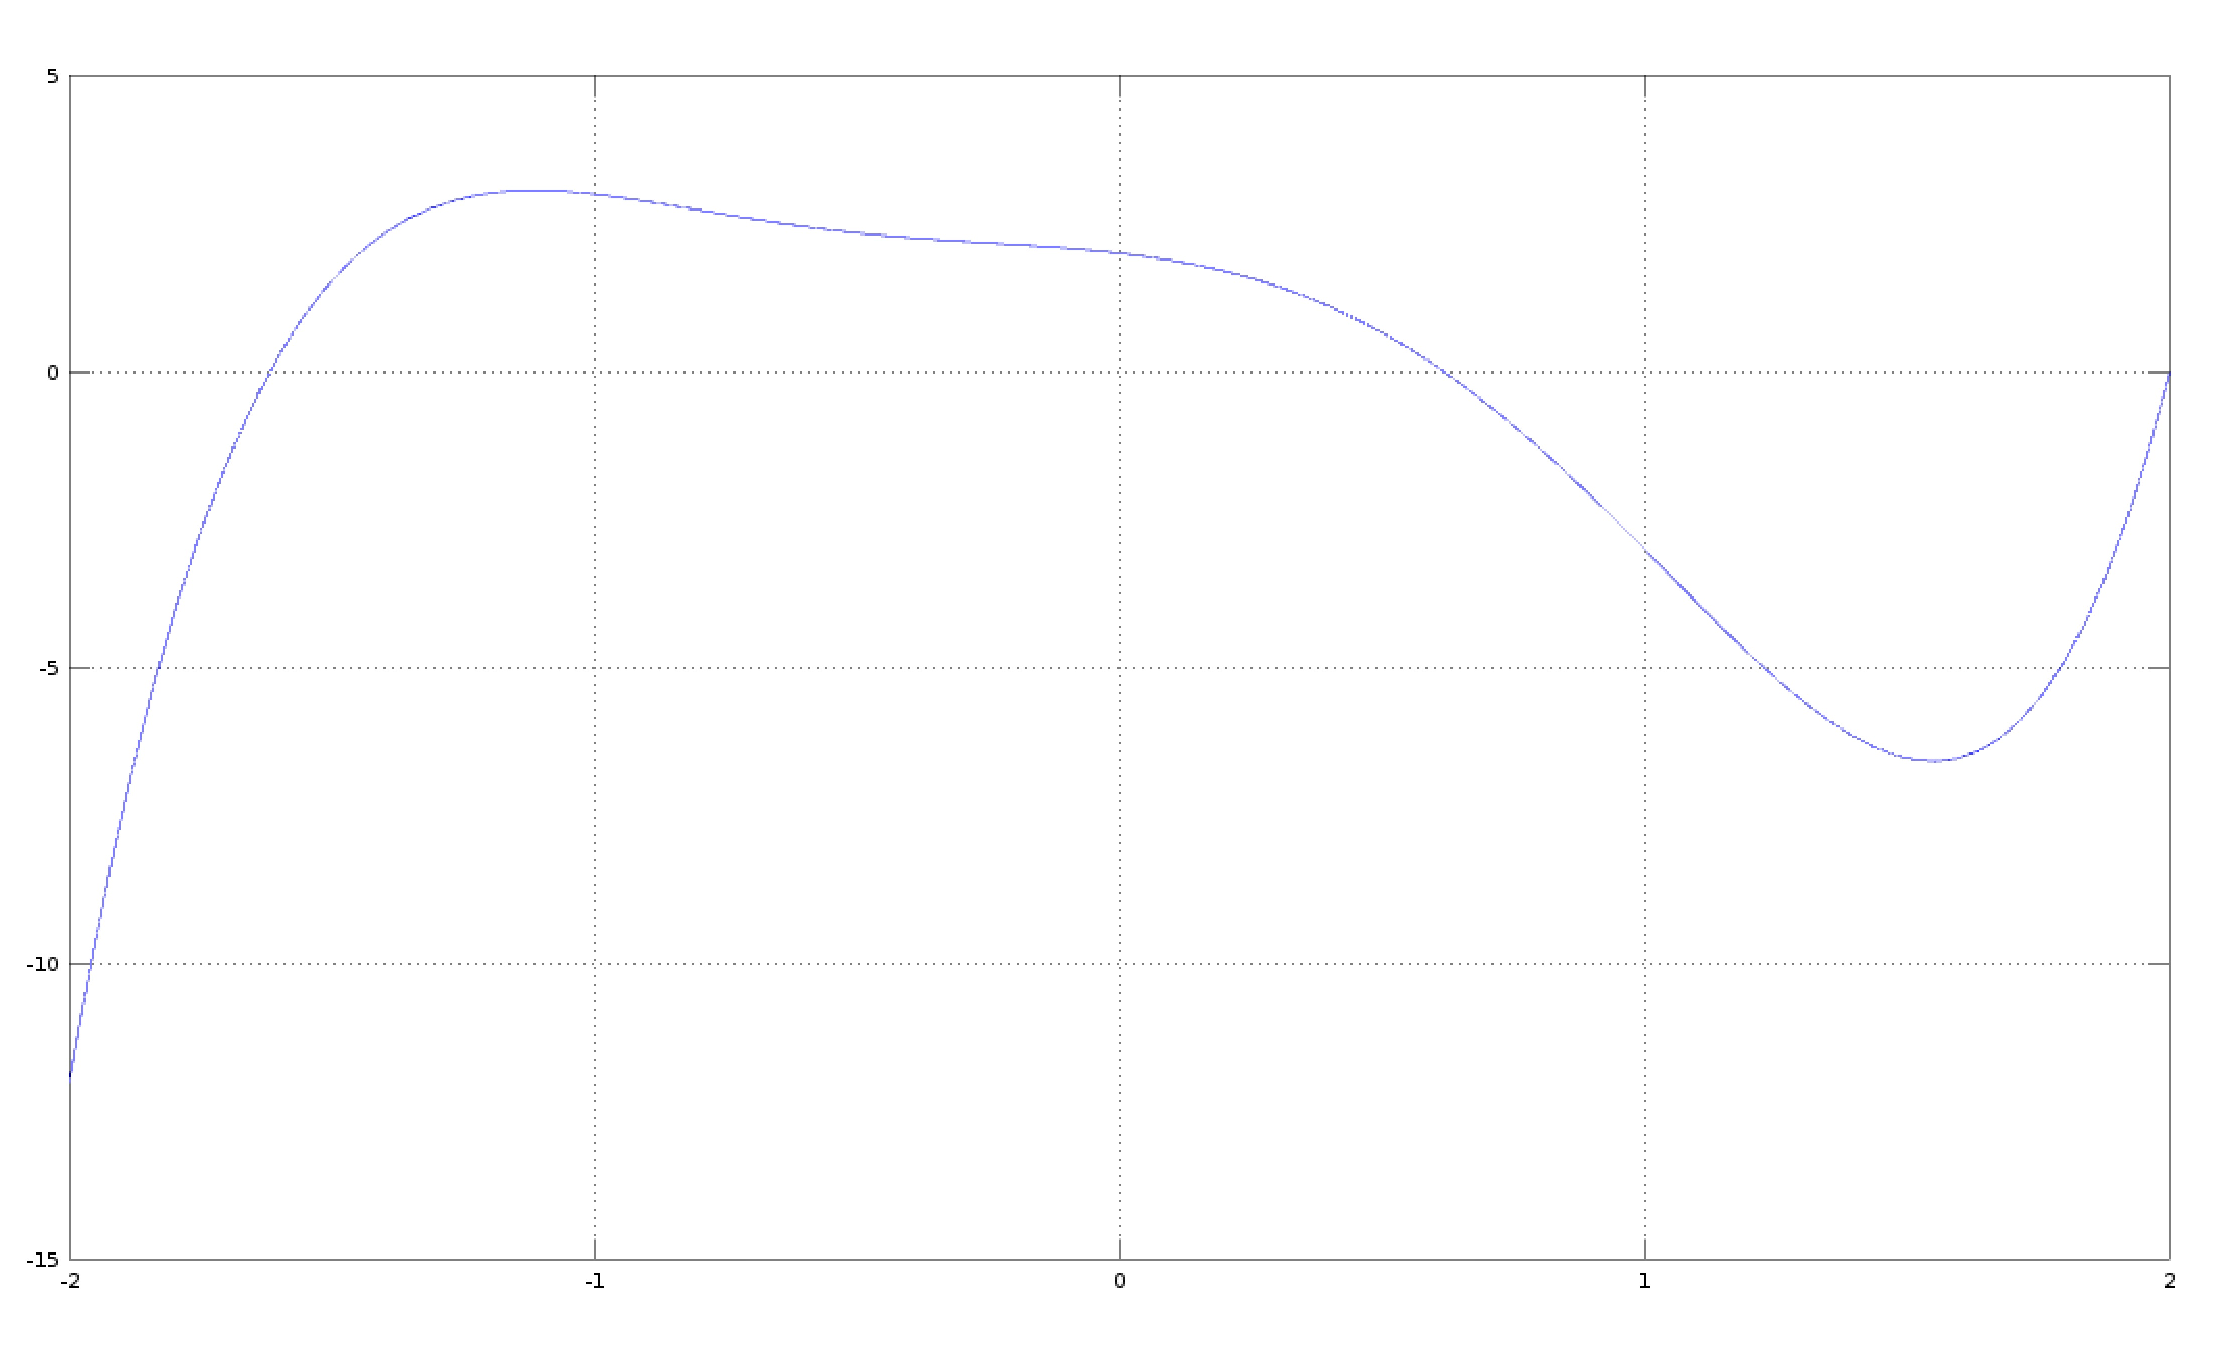
\includegraphics[scale = 0.3]{3.eps}
     \end{figure}
    \end{itemize}


    \subsection{Método de Bisección}
    
    \begin{itemize}
     \item $x-x^{x-cosx} = 0$ 
     
     Esta ecuación tiene varias respuestas dependiendo del intervalo que se le asigne.
     
     \begin{itemize}
      \item $a = 0.7$ $b = 1.2$
      \begin{figure}[h]
      \centering
      \includegraphics[scale = 0.4]{21.eps}
     \end{figure}
      
      \newpage
      
      \item $a = 1.1$ $b = 1.5$
      
      \begin{figure}[h]
      \centering
      \includegraphics[scale = 0.4]{212.eps}
     \end{figure}
      
     \end{itemize}

     
     
     
     
     
     \item $x-cos(senx) = 0$ $a = 0$ $b = 1$
      
      \begin{figure}[h]
      \centering
      \includegraphics[scale = 0.4]{22.eps}
     \end{figure}
     
     \item $x^5 - 3x^3 - 2x^2 + 2 = x$
     
     Esta ecuación tiene varias respuestas dependiendo del intervalo que se le asigne.
     
     
      \begin{itemize}
           
       \item $a = -2$ $b = -1$
      
      \begin{figure}[h]
      \centering
      \includegraphics[scale = 0.4]{231.eps}
     \end{figure}
      
      \newpage
       
       \item $a = 0$ $ b = 1$
       
       
       
      \begin{figure}[h]
      \centering
      \includegraphics[scale = 0.4]{232.eps}
     \end{figure} 
       
       \item $a = 1$ $b = 2$
       
	\begin{figure}[h]
      \centering
      \includegraphics[scale = 0.4]{233.eps}
     \end{figure} 
      \end{itemize}
    \end{itemize}

   
    
    
    \subsection{Método de Falsa Posición}
     
     \begin{itemize}
      \item $x-x^{x-cosx} = 0$
      
      Desde este punto solo se calculará el intervalo $a = 0.7$, $b = 1.2$ que dá la
     respuesta $1$ (La más cercana a cero):
     
     \begin{figure}[h]
      \centering
      \includegraphics[scale = 0.4]{31.eps}
     \end{figure}
     
     \item $x-cos(senx) = 0$ $a = 0$ $b = 1$
     
     \vspace{4.5mm}
      
      \begin{figure}[h]
      \centering
      \includegraphics[scale = 0.4]{32.eps}
     \end{figure}

     \item $x^5 - 3x^3 - 2x^2 + 2 = x$
     
     Desde este punto solo se calculará el intervalo $a = 0$, $b = 1$ que dá la
     respuesta $0.618033409118652$ (La más cercana a cero):
     
      \begin{figure}[h]
      \centering
      \includegraphics[scale = 0.4]{33.eps}
     \end{figure}
    \end{itemize}
 

 
    \subsection{Método de la Secante}
    
    \begin{itemize}
      \item $x-x^{x-cosx} = 0$ $r_{0} = 0.5$ $r_{1} = 0.8$
     
     \begin{figure}[H]
      \centering
      \includegraphics[scale = 0.6]{41.eps}
     \end{figure}

     \item $x-cos(senx) = 0$ $r_{0} = 0$ $r_{1} = 0.5$
     
      \begin{figure}[H]
      \centering
      \includegraphics[scale = 0.6]{42.eps}
     \end{figure}
    
     \item $x^5 - 3x^3 - 2x^2 + 2 = x$ $r_{0} = 0 $ $r_{1} =0.5 $
     
      \begin{figure}[h]
      \centering
      \includegraphics[scale = 0.6]{43.eps}
     \end{figure}
     
    \end{itemize}
   
  
  
    \subsection{Método de Newton}
    
    \begin{itemize}
    \item $x-x^{x-cosx} = 0$ $r_{0} = 0.5$
     
     \begin{figure}[h]
      \centering
      \includegraphics[scale = 0.6]{51.eps}
     \end{figure}
   
    
    \item $x-cos(senx) = 0$ $r_{0} = 1$
      
      \begin{figure}[h]
      \centering
      \includegraphics[scale = 0.6]{52.eps}
     \end{figure}
    
    \item $x^5 - 3x^3 - 2x^2 + 2 = x$ $r_{0} = 1$
     
      \begin{figure}[H]
      \centering
      \includegraphics[scale = 0.6]{53.eps}
     \end{figure}
    
    \end{itemize}

    
    \newpage
  
    \subsection{Método de Newton con derivada aproximada}
    
    \begin{itemize}
    \item $x-x^{x-cosx} = 0$ $r_{0} = 0.5$
     
     \begin{figure}[h]
      \centering
      \includegraphics[scale = 0.6]{61.eps}
     \end{figure}
   
    
    \item $x-cos(senx) = 0$ $r_{0} = 1$
      
      \begin{figure}[h]
      \centering
      \includegraphics[scale = 0.6]{62.eps}
     \end{figure}
    
    \item $x^5 - 3x^3 - 2x^2 + 2 = x$ $r_{0} = 1$
     
      \begin{figure}[h]
      \centering
      \includegraphics[scale = 0.6]{63.eps}
     \end{figure}
    
    \end{itemize}

    \subsection{Método del Punto Fijo}
    
    \begin{itemize}
    \item $x-x^{x-cosx} = 0$ $r_{0} = 0.7$
     
     \begin{figure}[H]
      \centering
      \includegraphics[scale = 0.6]{71.eps}
     \end{figure}
   
   \newpage
    
    \item $x-cos(senx) = 0$ $r_{0} = 1$
      
      \begin{figure}[h]
      \centering
      \includegraphics[scale = 0.6]{72.eps}
     \end{figure}
    
    \end{itemize}
    
    
\end{document}
